\documentclass[]{scrartcl}

\usepackage{amsmath}
\usepackage{amssymb}
\usepackage[utf8]{inputenc}
\usepackage[T1]{fontenc}
\usepackage{lmodern}
\usepackage{ngerman}
\usepackage{geometry}
\usepackage{graphicx}
\usepackage{wrapfig}
\usepackage{caption}
\usepackage{wasysym}
\usepackage{siunitx}
\usepackage{picinpar}
\usepackage{tikz}
\usepackage{float}

\renewcommand{\figurename}{Abb.}
\usepackage[
	colorlinks=true,
	urlcolor=blue,
	linkcolor=black
]{hyperref}


%Hier Titel und so
\newcommand{\versuchnummer}{Nummer} 
\newcommand{\versuchname}{Name} 
\newcommand{\versuchdatum}{Datum} 


\title{Versuch \versuchnummer\\ \versuchname}
\subtitle{Physikalisches Fortgeschrittenenpraktikum}
\author{Robert Rauter und Björn Lindhauer}
\date{\versuchdatum} 
\begin{document}
\begin{titlepage}
{\large \versuchdatum}
\vspace{7cm}
\begin{center}
\textbf{\huge Versuch \versuchnummer}{V56}\\
\vspace{0.5cm}
\textbf{\huge \versuchname}{Modulation und Demodulation elektrischer Schwingungen}\\
\vspace{0.2cm}
\textbf{ Physikalisches Fortgeschrittenenpraktikum}\\
\vspace{9cm}

{\Large Robert Rauter \ \ \hspace{1.5cm} und \hspace{1.5cm} Björn Lindhauer}\\
{ \url{robert.rauter@tu-dortmund.de} \ \ \hspace{2cm} \url{bjoern.lindhauer@tu-dortmund.de}}
\end{center}
\end{titlepage}
\section{Einleitung}
Unter Modulation wird Veränderung der Amplitude, der Phase oder der Frequenz einer Welle im Rhythmus des Nachrichtensignals verstanden. Sie wird benötigt, um Signale mit elektromagnetische Wellen zu übertragen.\\
Das übertragene Signal muss beim Empfänger anschließend zurück gewonnen werden. Dieser Vorgang wird als Demodulation bezeichnet.\\ Mit der Zeit wurden verschiedene Verfahren mit unterschiedlichen Stärken und Schwächen in der Störsicherheit, im Wirkungsgrad, in der Verzerrungsfreiheit und in der Breite des Frequenzspektrums entwickelt. Diese Verfahren lassen sich in zwei Klassen, den Amplitudenmodulations- und Phasenwinkelmodulation- Verfahren unterteilen.\\
In diesen Versuch sollen Beispiele beider Verfahrensklassen untersucht werden.
\section{Theoretische Grundlagen}
\subsection{Amplitudenmodulation}
Eine Amplitudenmodulation kann durch eine hochfrequente Trägerschwingung $U_{\text{T}}\left(t\right)$ mit niederfrequenten Modulationssignal $U_{\text{M}}\left(t\right)$ erreicht werden.
-
\begin{align}
U_{\text{T}}\left(t\right)=\hat{U}_{\text{T}} \cos \omega_{\text{T}}t  \text{, }U_{\text{M}}\left(t\right)=\hat{U}_{\text{M}} \cos \omega_{\text{M}}t
\end{align}
Resultierende amplitudenmodulierte Schwingung:
\begin{align}
U_3\left(t\right)=\hat{U}_{\text{T}} \left(1+m\cos \omega_{\text{U}}t\right)\cos \omega_{\text{T}}t
\end{align}
\begin{figure}[H]
\centering 
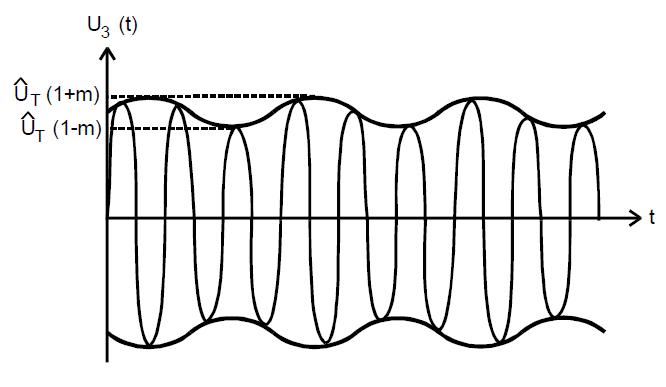
\includegraphics[width=10cm]{images/zeitabhaengigkeit_momentanspannung.png}
\label{fig:zeitabhaengigkeit_momentanspannung}
\caption{Text}
\end{figure}

\section{Durchführung}

\section{Auswertung}

\subsection{Amplitudenmodulation mit Ringmodulator}
Mit einem Ringmodulator wird ein amplitudenmoduliertes SignaL mit Trägerunterdrückung erzeugt. Freequenzen f und Amplituden U von Träger- und Modulationssignal lauten:
\begin{enumerate}
	\item Trägersignal
	\item Modulationssignal 
\end{enumerate}
\subsection{Amplitudendemodulation mit Ringmodulator}

\subsection{Amplitudenmodulation mit Diode}

\subsection{Amplitudendemodulation mit Diode}

\subsection{Frequenzmodulation}

\subsection{Frequenzdemodulation}

\section{Diskussion}

\section{Quellen}

\end{document}